% Base template source: https://tex.stackexchange.com/questions/8827/preparing-cheat-sheets

\documentclass[10pt,landscape]{article}

\usepackage{multicol}
\usepackage{lipsum}

\usepackage{calc, ifthen,hyperref, gensymb, comment, textcomp}
\usepackage{amsmath,amsthm,amsfonts,amssymb,geometry}
\usepackage{color,graphicx,overpic}

% This sets page margins to .5 inch if using letter paper, and to 1cm
% if using A4 paper. (This probably isn't strictly necessary.)
% If using another size paper, use default 1cm margins.
\ifthenelse{\lengthtest { \paperwidth = 11in}}
    { \geometry{top=.25in,left=.25in,right=.25in,bottom=.25in} }
    {\ifthenelse{ \lengthtest{ \paperwidth = 297mm}}
        {\geometry{top=1cm,left=1cm,right=1cm,bottom=1cm} }
        {\geometry{top=1cm,left=1cm,right=1cm,bottom=1cm} }
    }

% Turn off header and footer
\pagestyle{empty}

% Don't print section numbers
\setcounter{secnumdepth}{0}

% Define Image
\newenvironment{Figure}
     {\par\medskip\noindent\minipage{\linewidth}}
     {\endminipage\par\medskip}
    
% Define Line Spacing
\linespread{.3}
% -----------------------------------------------------------------------

\begin{document}
\raggedright
\footnotesize

% Area Above Columns
\begin{center}
     \Large{\underline{Heat Transfer - Zak Olech - 9/19/2019}}
\end{center}
\begin{multicols}{3}

% multicol parameters
% These lengths are set only within the two main columns
\setlength{\columnseprule}{0.25pt}
\setlength{\premulticols}{1pt}
\setlength{\postmulticols}{1pt}
\setlength{\multicolsep}{1pt}
\setlength{\columnsep}{2pt}

\begin{comment}
\section{Variables (Alphbetical By Variable)}


% -----------------------------------------------------------------------
\section{General Information}
\subsection{Conversion Factors}

\subsection{Process}
1 - Assumptions\\*
2 - Properties\\*
3 - Analysis\\*
\subsection{Assumptions}
\subsection{Metric Prefix}
\begin{Figure}
    \centering
    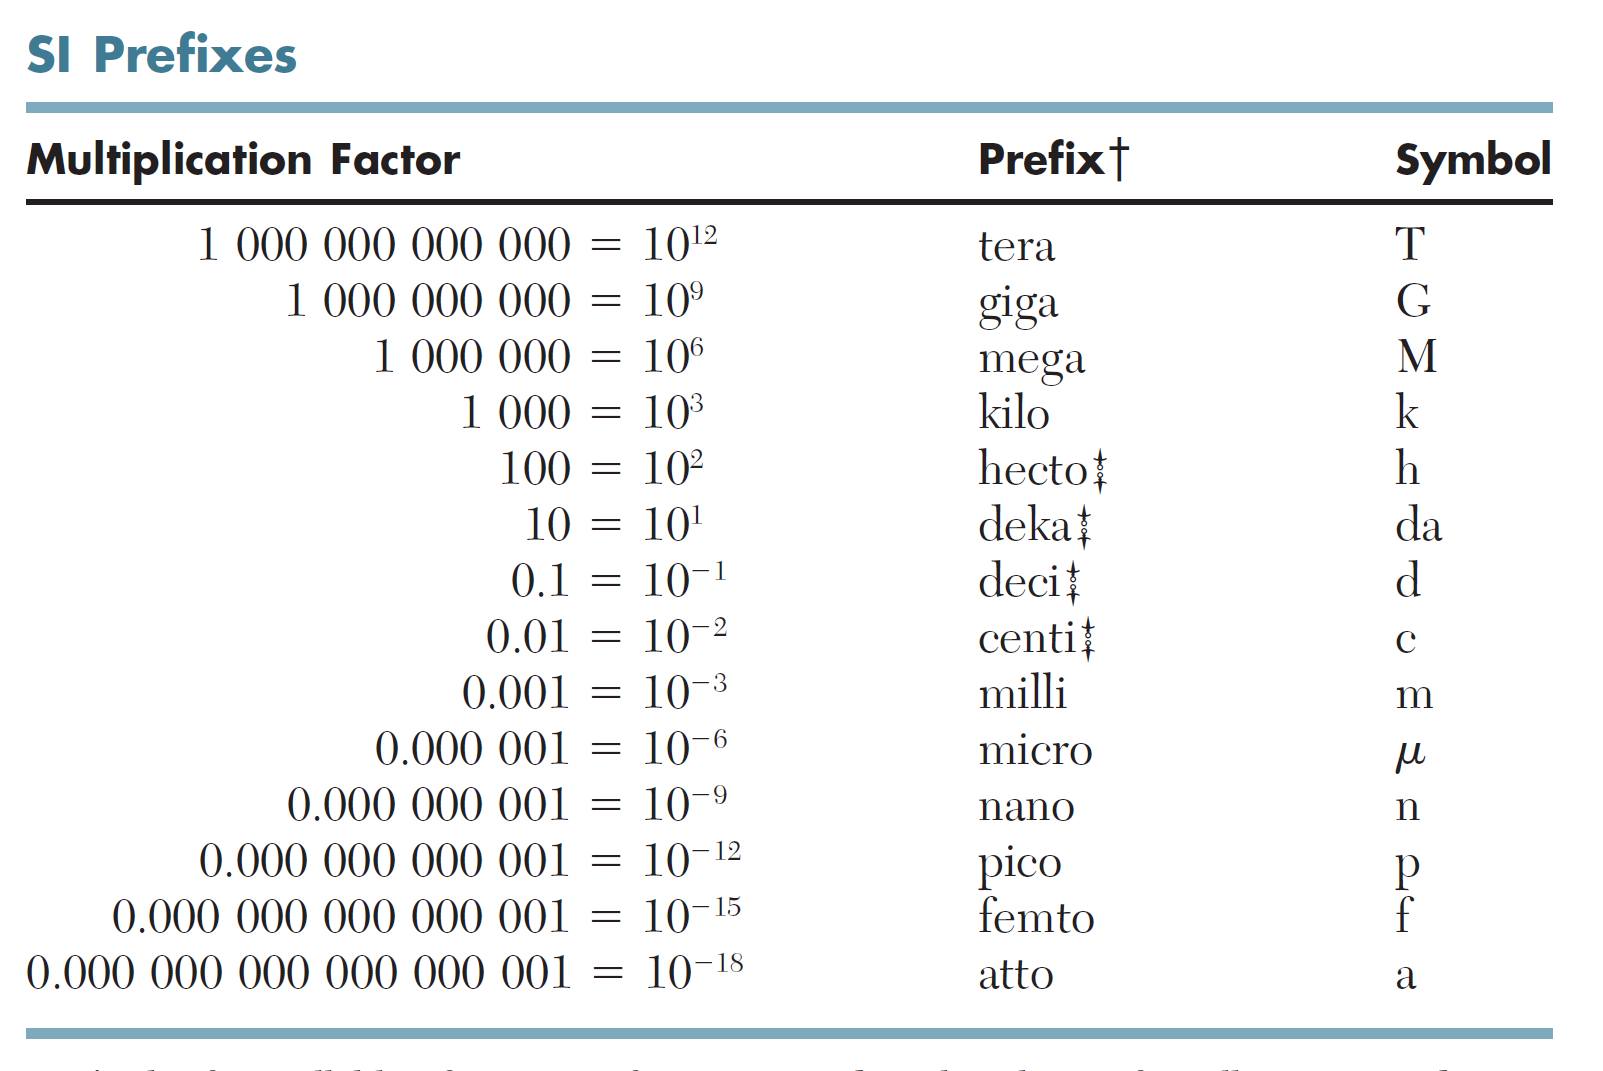
\includegraphics[width=\linewidth, height=8cm]{SI_Prefix.png}
\end{Figure}

\section{Chapter 1 - Introduction}
\subsection{1 - What and how}
\subsection{2 - Physical Origins and Rate Equations}
\subsection{3 - Relationship to Thermodynamics}
%\subsection{4 - Units and Dimensions}
%\subsection{5 - Analysis of Heat Transfer Problems: Methodology}
%\subsection{6 - Relevance of Heat Transfer}

\section{Chapter 2 - Introduction to Conduction}
\subsection{1 - The Conduction Rate Equation}
\subsection{2 - The Thermal Properties of Matter}
\subsection{3 - The Heat Diffusion Equation}
\subsection{4 - Boundary and Initial Conditions}

\section{Chapter 3 - One-Dimensional Steady-State Conduction}
\subsection{1 - The Plane Wall}
\subsection{2 - An Alternative Conduction Analysis}
\subsection{3 - Radial Systems}
\subsection{4 - Summary of One-Dimensional Conduction Results}
\subsection{5 - Conduction with Thermal Energy Generation}
\subsubsection{Ohmic heating}
\begin{equation}
    \dot{q}=\frac{\dot{E}_g}{\forall}=\frac{I^2R_e}{\forall}
\end{equation}
\subsubsection{Absorption of Radiation}
\begin{equation}
     \dot{q}\varproptoe^{-\alpha x}
\end{equation}
\subsubsection{The Plane Wall}
Heat Equation\\*
\begin{equation}
    \frac{d}{dx}(k\frac{dT}{dx})+\dot{q}=0\rightarrow\frac{d^2T}{dx^2}+\frac{\dot{q}}{k}=0
\end{equation}
General Solution\\*
Symmetric Surface Conditions\\*
- Temperature Distribution\\*
- Overall Energy Balance\\*
\subsubsection{Radial Systems}
Cylindrical (Tube) Wall\\*
Solid Cylinder (Circular Rod)\\*
- Heat Equation (Cylindrical)
Spherical Wall (Shell)\\*
Solid Sphere\\*
- Heat Equation (Spherical)\\
\subsection{6 - Extended Surfaces}


\section{Appendix}
\subsection{Appendix C.}

%\subsection{6 - Heat Transfer from Extended Surfaces}
%\subsection{7 - The Bioheat Equation}
%\subsection{8 - Thermoelectric Power Generation}
%\subsection{9 - Micro- and Nanoscale Conduction}


% References
%\rule{0.3\linewidth}{0.25pt}
%\scriptsize
%\bibliographystyle{abstract}
%\bibliography{Bibliography}

% End of document
\end{multicols}
\end{document}